\scanpage{359}
\mspage{EZ 2}
Cor
\diagram{\begin{tikzcd}[ampersand replacement=\&]
\Sigma_n\arrow[r] \& E\Sigma_n=\deleted{\unsure{K(\Sigma_n,1)}}\arrow[d,no head]\\
\& K(\Sigma_n,1)
\end{tikzcd}}
\[
W_n=\mathbb ZE\Sigma_n\xrightarrow{\sim}\mathbb Z
\]
\inserted{résol de \(\mathbb Z\) par des \(\Sigma_n\)-modules \deleted{plats} libres.}

Cor du th
\[
W_n\xrightarrow{\unsure{\urcorner|?|\sim}}\mathrm{Hom}^{\unsure{'|\bullet}}(\deleted{\unsure{\mathbb ZX\otimes\mathbb ZX}}\;\mathbb ZX\times X\times\ldots,\ \mathbb ZX\otimes\ldots\otimes\mathbb ZX)
\]
D'où par adjonction une fleche
\[
\begin{aligned}
W_n\otimes\mathbb Z(X\times\ldots\times X)&\xrightarrow{\lambda}\mathbb ZX\otimes\mathbb ZX\ldots\otimes\mathbb ZX\\
(\text{resp. }W_n\otimes\mathbb ZX\otimes\ldots\otimes\mathbb ZX&\longrightarrow\mathbb Z(X\times\ldots\times X)\;)
\end{aligned}
\]
Ceci exprime l'homotopie-commutativité \unsure{enoncée|annoncée} \(+\) haut

\uline{Ex \(n=2\)}\quad 1) exemple topologique :
\[
\begin{aligned}
X\times X&\xrightarrow{m} X\qquad\text{homotopiq com}\\
\Sigma_2\ \text{équiv}\quad I\times X\times X&\longrightarrow X \qquad\ldots\longrightarrow\\
+\ \text{fort}\quad E\Sigma_2\times X^2&\longmapsto X\qquad \Sigma_2\ \text{equiv}
\end{aligned}
\]
classiquemen \(\quad E\Sigma_n\times X^n\longrightarrow X\)\quad relevant la mult itérée

\(\Sigma_2\) agit sur \(S^n\) par action antipodale
\[
\begin{aligned}
&\downarrow\hspace{4em} E\Sigma_2=\varinjlim S^n\\
&\mathbb P^n(\mathbb R)\qquad x,y\qquad\deleted{xy=yx}\\
&&xyx^{-1}y^{-1}
\end{aligned}
\]
\diagram{\begin{tikzcd}[ampersand replacement=\&]
S^1\times X^2\arrow[r]\arrow[d] \& X\\
S^2\times X^2\arrow[ur,"\Sigma_2\text{-equiv}"] \&
\end{tikzcd}}
etc \ldots

\figure{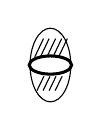
\begin{tikzpicture}[scale=.55]
\draw (0,0) ellipse (.47 and .85);
\draw[line width=1.1pt] (0,0) ellipse (.49 and .21);
\foreach \a in {-0.28,-0.15,0,.14,.27}{\draw (\a-.08,.19) -- (\a+.12,.61);}
\foreach \a in {-.23,-.09,.05,.19}{\draw (\a-.08,-.59) -- (\a+.08,-.26);}
\end{tikzpicture}}

\(\Sigma_n\times\Sigma_n=\Sigma_n\)
\diagram{\begin{tikzcd}[ampersand replacement=\&]
{\deleted{\unsure{E\Sigma_n\times(E\Sigma_j\times X^j)^n|E\Sigma_n\times(E\Sigma_j\times X)^n}}}\arrow[d] \&
{E(\Sigma_n\int\Sigma_j)\times(X_1^0\ldots X_j^0)\times X_1^1\ldots X_j^1\times\ldots X_1^n\times\ldots\times X_{j}^n}\arrow[l]\arrow[dd]\\
X^n \& {}\\
X \& E\Sigma_n\times X^n\arrow[l,"?"']
\end{tikzcd}}
Cor : les enoncés précédents impliquent que lorsque \(X\) est un H esp sat à ce genre de cdn de commutativité à homotopie près, alors les chains \(\mathbb ZX\) ont ce
\[
W_n\otimes\mathbb ZX^{\otimes n}\xrightarrow{\Sigma_n\ \text{equiv}}\mathbb ZX^{\unsure{\epsilon|e|\otimes}}\longrightarrow
\]
t.q induise la mult des chains
\[
\mathbb ZX^{\otimes n}\xrightarrow[\text{shuffles}]{EZ}\mathbb Z(X^n)\xrightarrow{\mathbb Z(m)}\mathbb ZX
\]
Constr des operations de Steenrod :
\[
\mathbb ZX\unsure{\longrightarrow|\rightrightarrows}\qquad A\ \text{un anneau de car}\ p
\]
\[
\deleted{\unsure{f\in}}Z^n(X,A)\qquad(\widetilde{\mathbb ZX})\xrightarrow{f} A[n]
\]
\diagram{\begin{tikzcd}[ampersand replacement=\&,column sep=small]
W_p\otimes\mathbb Z(X^p)\arrow[r,"\lambda"] \& \widetilde{\mathbb ZX}^{\otimes p}\arrow[r,"f^{\otimes p}"] \& A[n]^{\otimes p}\arrow[r,"\mu"] \& A[pn]\\
W_p\otimes\mathbb ZX\arrow[u,"\Delta"]\arrow[urrr,"\Sigma_n\ \text{equiv}"'] \& \& \&
\end{tikzcd}}
\margin{\fbox{\(\substack{\text{cf Steenrod p \uline{39}}\\ \text{\uline{Coh} ops}}\)}}

(avec action triv sur \(\mathbb ZX\))
\(\deleted{\unsure{W_{\Sigma_n}}}\)
\[
\begin{aligned}
Pf&=\mu\circ f^{\times p}\circ\lambda\ \in{}_{\Sigma_n}H^{pn}(\mathbb Z(X^p),A)\\
&\hspace{12em}\downarrow\\
\bigl(W_n\otimes\mathbb ZX/\Sigma_n&=\mathbb ZX\otimes\mathbb ZK(\Sigma_n,1)\qquad{}_{\Sigma_n}H^{\unsure{p\times n|pn}}(X,A)\\
\Sigma_n&\hspace{14em}\shortparallel\\
&\hspace{9em}H^*(K(\Sigma_{p})\deleted{\unsure{\times}}\times X,A)\\
&\hspace{14em}\shortparallel\\
\text{Kunneth}\quad &H^*(\Sigma_p)\otimes_{\mathbb F_p}H^*(X,A)
\end{aligned}
\]
% archive sheet number: 360
